\def\QRCODE{TB_IPR_TUT.IMG.granulometry_pythonqrcode.png}
\def\QRPAGE{http://www.iptutorials.science/tree/master/TB_IPR/TUT.IMG.granulometry/python}
\pcorrectionsection{Python correction}
\subsection{Simulation}
The construction of an homothetic structuring element is necessary for computing a granulometry (through the function \pinline{iterate_structure}.

\begin{python}
def granulometry(BW, T=35):
    # total original area
    A = ndimage.measurements.sum(BW);
    
    # number of objects
    label, N = ndimage.measurements.label(BW);
    
    area=np.zeros((T,), dtype=np.float);
    number=np.zeros((T,), dtype=np.float);
    
    """
    Warning: the structuring elements must verify B(n) = B(n-1) o B(1).
    """
    se = ndimage.generate_binary_structure(2, 1);
    for i in np.arange(T):
        SE = ndimage.iterate_structure(se, i-1);
        m = ndimage.morphology.binary_erosion(BW, structure=SE);
        G = ndimage.morphology.binary_propagation(m, mask=BW);
        area[i]=100*ndimage.measurements.sum(G)/A
        label, n = ndimage.measurements.label(G);
        number[i] = 100*n/N; # beware of integer division
    
    plt.figure()
    plt.plot(area, label='Area')
    plt.plot(number, label='Number')
    plt.legend()
    #plt.savefig("granulo_poudre1.pdf");
    plt.show()
    
    plt.figure();
    plt.plot(-np.diff(area), label='Area derivative');
    plt.plot(-np.diff(number), label='Number derivative');
    plt.legend()
    #plt.savefig("granulo_poudre2.pdf");
    plt.show()
\end{python}

The results are shown in Fig. \ref{fig:granulo:python:simu}, generated by the following code:
\begin{python}
## Granulometry of synthetic image
# read binary simulated image, normalize it
I = imageio.imread("simulation.png")/255;
I = I[:,:,2]>.5;
plt.figure();
plt.imshow(I);
plt.show();

granulometry(I, 35);
\end{python}

\begin{figure}[H]
\centering\caption{Granulometry on simulated image.}%
 \subfloat[Simulated image of disks.]{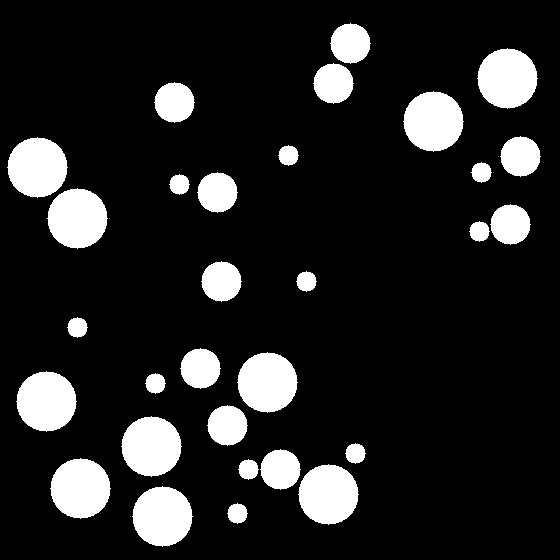
\includegraphics[width=.4\linewidth]{simulation.png}}
 
 \subfloat[Granulometry in number and area.]{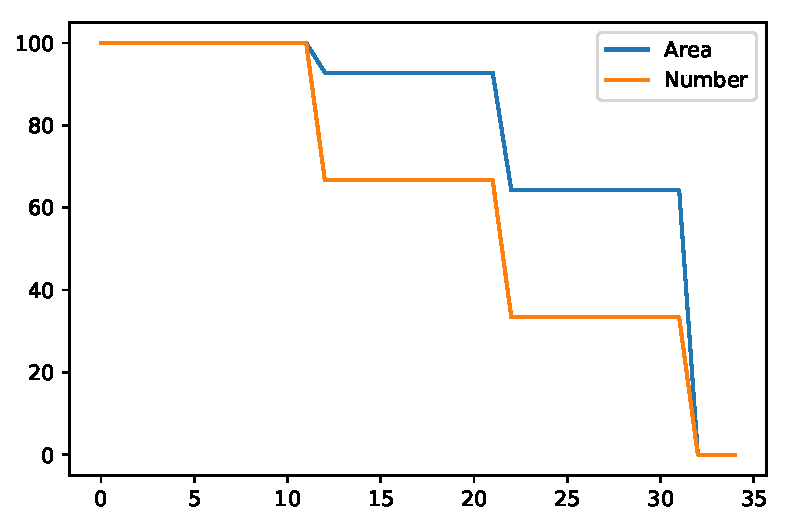
\includegraphics[width=.45\linewidth]{granulo_simu1.pdf}}\hfill
 \subfloat[Derivatives.]{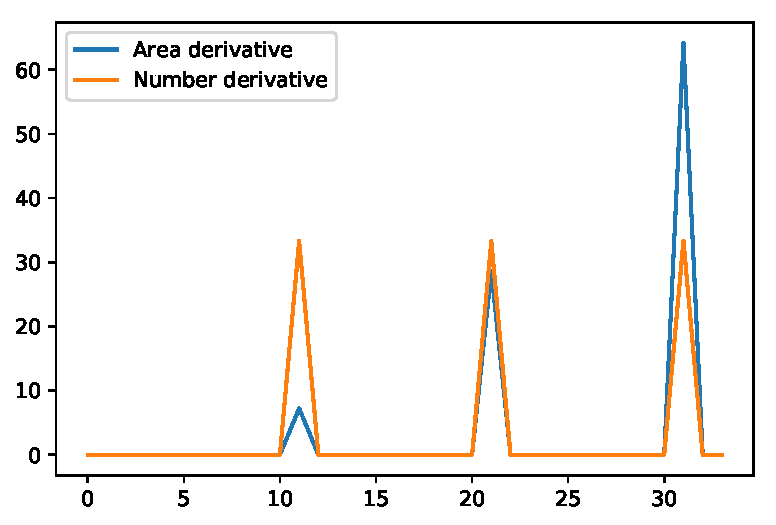
\includegraphics[width=.45\linewidth]{granulo_simu2.pdf}}%
 \label{fig:granulo:python:simu}%
\end{figure}


\subsection{Powder image and segmentation}

First of all, the image must be binarized, i.e. segmented. The following code is a proposition of segmentation, leading to the result presented in Fig. \ref{fig:granulo:python:poudre:segmentation}.

\begin{python}
## Granulometry of real image
I = imageio.imread("poudre.bmp");

# segmentation
BW = I>74;
BW = ndimage.morphology.binary_fill_holes(BW);

# suppress small objects
se = ndimage.generate_binary_structure(2, 1);
m = ndimage.morphology.binary_opening(BW);
# opening by reconstruction
BW=ndimage.morphology.binary_propagation(m, mask=BW);

imageio.imwrite("segmentation.png", BW);
plt.imshow(BW)
plt.show()

granulometry(BW, 20);
\end{python}


\begin{figure}[htbp]
\centering\caption{Results of granulometry analysis of original image from \protect\subref{fig:granulo:python:poudre}.}%
\subfloat[Original image of powder.]{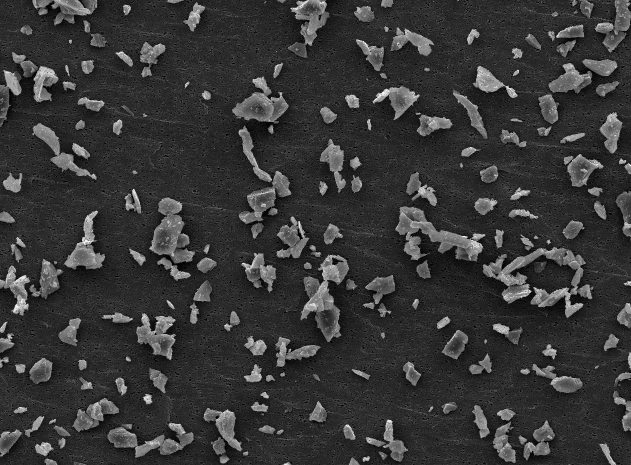
\includegraphics[width=.45\linewidth]{poudre.png}\label{fig:granulo:python:poudre}}\hfill
\subfloat[Segmentation of image of \protect\subref{fig:granulo:python:poudre}.]{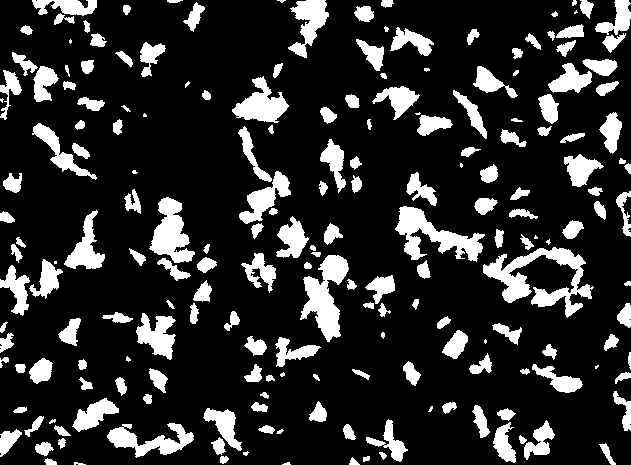
\includegraphics[width=.45\linewidth]{segmentation_granulo.python.png}}

\subfloat[Granulometry.]{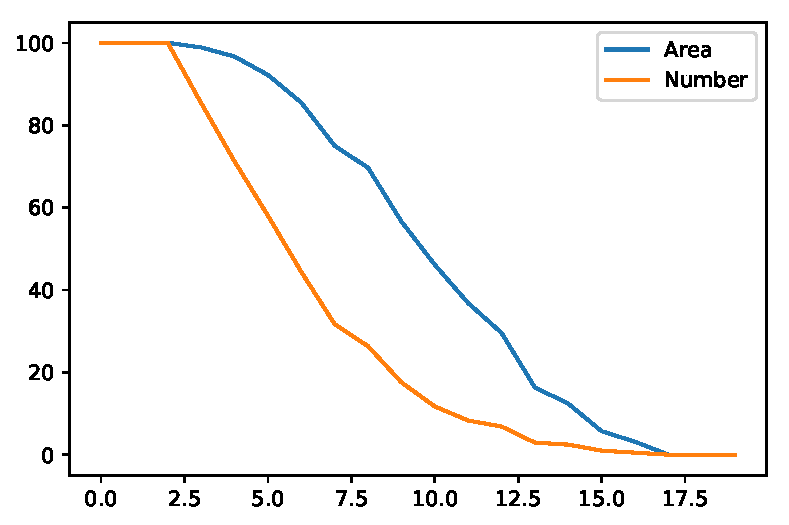
\includegraphics[width=.45\linewidth]{granulo_poudre1.pdf}\label{fig:granulo:python:poudre:segmentation}}
\hfill
\subfloat[Derivative.]{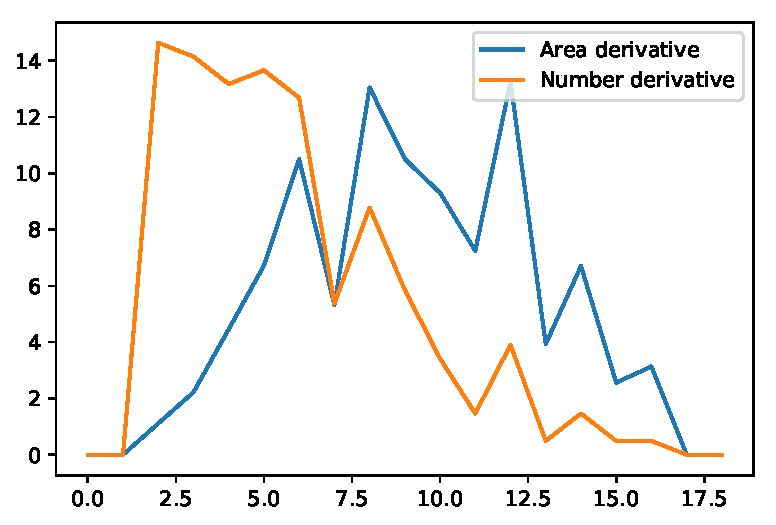
\includegraphics[width=.45\linewidth]{granulo_poudre2.pdf}}%
 \label{fig:granulo:python:poudre:granulo}%
\end{figure}
